\section{SPH方法数学基础}

\subsection{$\delta$ 函数与光滑函数}

\begin{frame}
    $\delta$ 函数是一个由积分性质定义的特殊函数,在一维情况下其定义为:
    \begin{equation}
        \begin{aligned}
            &\delta(x) = \begin{cases}
                +\infty, & x = 0 \\
                0, & x \neq 0
            \end{cases}
            \\
            &\int_{-\infty}^{+\infty} \delta(x) \mathrm{d}x = 1
        \end{aligned}
    \end{equation}

    其具有两个重要的性质:

    \begin{itemize}
        \item 紧致性:$\delta(x) = 0, \forall x \neq 0$
        \item 筛选性:$\int_{-\infty}^{+\infty} f(\xi) \delta(x - \xi) \mathrm{d}\xi = f(x)$
    \end{itemize}

    上述两个性质是SPH方法产生的数学基础,
    根据紧致性和筛选性质,
    我们可以根据 $\delta$ 函数的这两个性质构造一个与之类似的光滑函数(或者称核函数) $W(x;h)$ ,
    其应该满足:
    \begin{equation}
        \begin{aligned}
            &W(x;h) = 0, \forall |x| > th\\
            &\int_{-\infty}^{+\infty} W(x;h) \mathrm{d}x = 1
        \end{aligned}
    \end{equation}
\end{frame}

\begin{frame}
    这里给出一个核函数的例子:
    \begin{equation}
        W(\vec{r};h) = \begin{cases}
            \frac{315}{64\pi h^9} (h^2 - |\vec{r}|^2)^3, & 0 \leq |\vec{r}| \leq h \\
            0, & |\vec{r}| > h
        \end{cases}
    \end{equation}

    \begin{figure}[H]
        \centering
        \subfigure[$\delta(x)$ 函数]{
            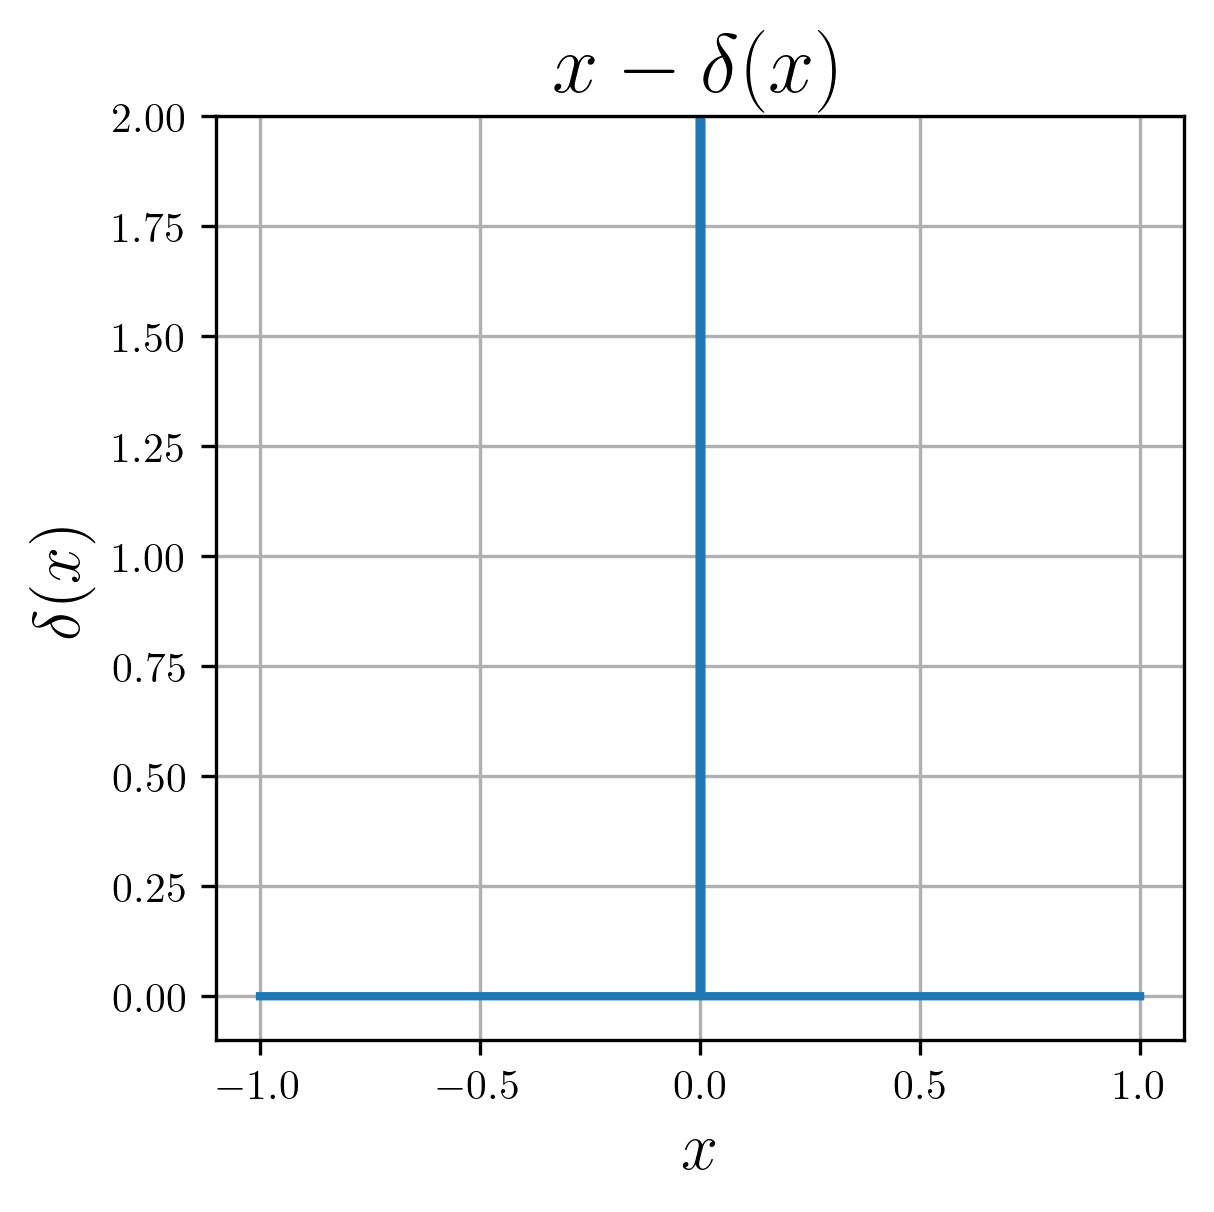
\includegraphics[width=0.3\textwidth]{images/delta.png}
        }
        \qquad
        \subfigure[光滑核函数(一维剖面)]{
            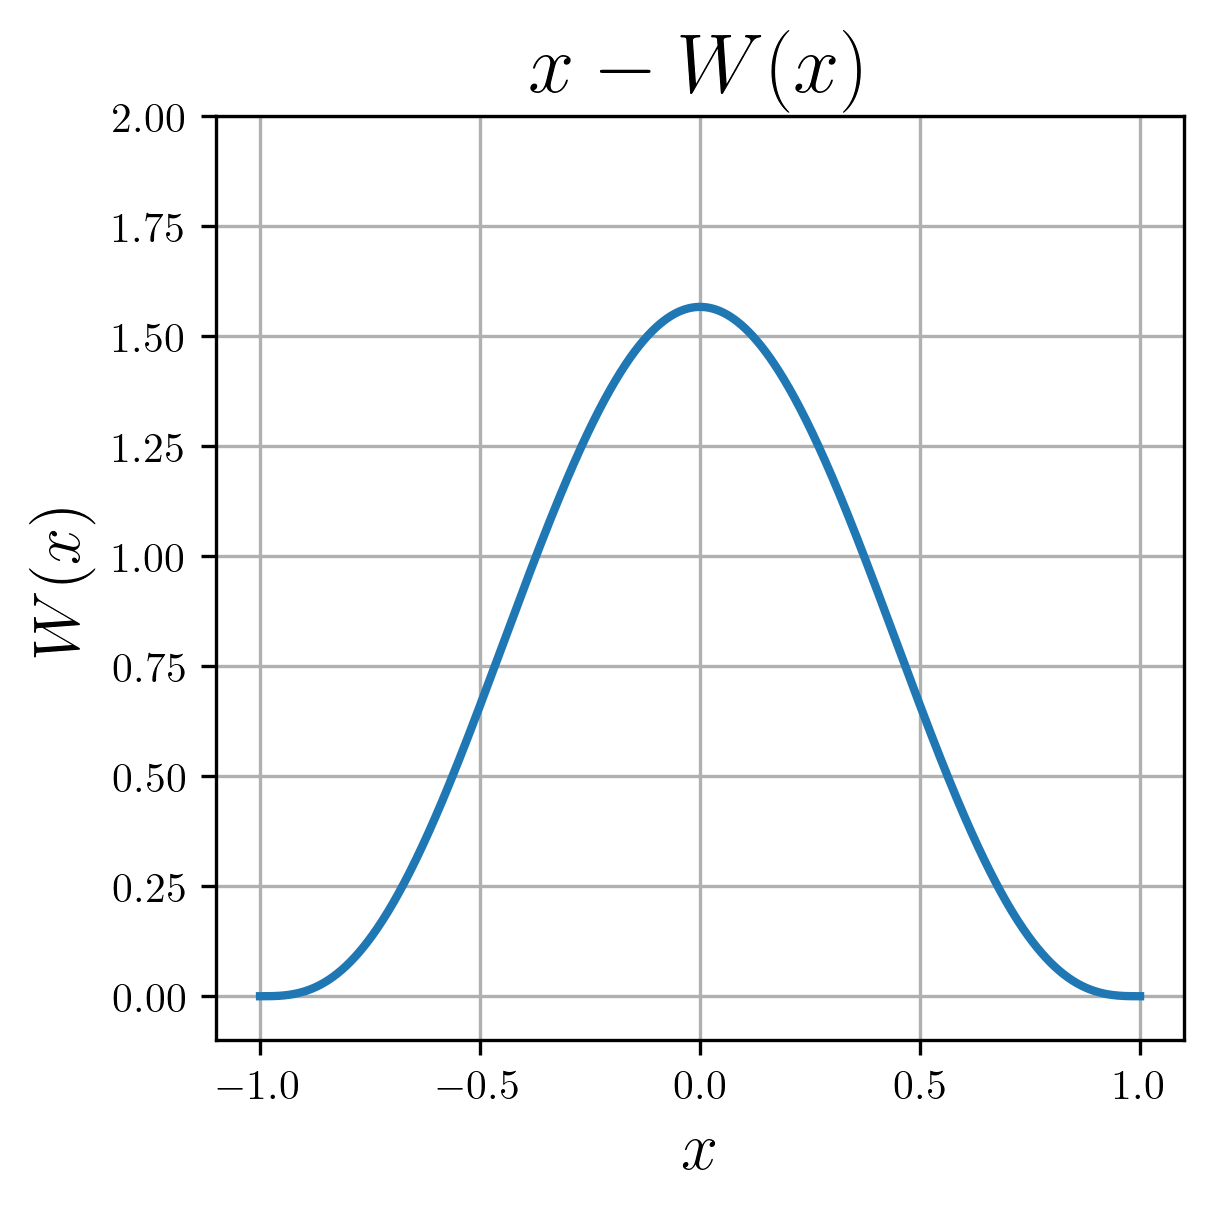
\includegraphics[width=0.3\textwidth]{images/W.png}
        }
        \caption{$\delta$ 函数与光滑核函数的示意图}
    \end{figure}

    这里需要补充说明的是,在编程实践中 $h$ 表示核半径,
    $t$ 表示核半径的某个倍数,数学推导中取 $t = 1$ 。
\end{frame}

\begin{frame}
    根据 $\delta$ 函数的两个性质,我们可以用 $W$ 光滑函数导出如下两个近似:

    \begin{itemize}
        \item 筛选性:
        \begin{equation}
            u(\vec{r})\approx \int_{\Omega} u(\vec{r}^\prime) 
            W(\vec{r} - \vec{r}^\prime;h) \mathrm{d}\vec{r}^\prime
        \end{equation}
        \item 紧致性:
        \begin{equation}
            \begin{aligned}
                \nabla u(\vec{r}) &\approx \int_{\Omega} \nabla u(\vec{r}^\prime)
                W(\vec{r} - \vec{r}^\prime;h) \mathrm{d}\vec{r}^\prime \\
                &=
                \int_{\partial\Omega} u(\vec{r}^\prime) \vec{n}(\vec{r}^\prime)
                W(\vec{r} - \vec{r}^\prime;h) \mathrm{d}S^\prime - 
                \int_{\Omega} u(\vec{r}^\prime) \nabla^\prime
                W(\vec{r} - \vec{r}^\prime;h) \mathrm{d}\vec{r}^\prime\\
                &\mathop{=}^{\text{紧致性}} -\int_{\Omega} u(\vec{r}^\prime) \nabla^\prime
                W(\vec{r} - \vec{r}^\prime;h) \mathrm{d}\vec{r}^\prime
            \end{aligned}
        \end{equation}
    \end{itemize}

    上述两个式子是SPH方法的数学基础,表明某个标量场 $u(\vec{r})$ 
    和其在该点的梯度 $\nabla u(\vec{r})$ 可以用该点附近的标量场值在光滑核函数加权下的积分来近似。
\end{frame}

\subsection{物质点的离散}

\begin{frame}
    我们先考虑标量场 $u(\vec{r})$ 值的近似,假设我们有 $N$ 个物质点,
    任意分布在 $\Omega$ 区域内,其位置分别为 $\vec{r}_i, i = 1, 2, \cdots, N$ ,
    则标量场 $u(\vec{r})$ 在 $\vec{r}_i$ 处的近似值为:
    \begin{equation}
        \label{eq:scalar_field_approximation}
        \begin{aligned}
            u(\vec{r})&\approx \int_{\Omega} u(\vec{r}^\prime) 
                W(\vec{r} - \vec{r}^\prime;h) \mathrm{d}\vec{r}^\prime\\
            &\approx
            \sum_{j=1}^{N} u_j W(\vec{r} - \vec{r}_j;h) V_j\\
            &=
            \sum_{j=1}^{N} u_j W(\vec{r} - \vec{r}_j;h) \frac{m_j}{\rho_j}
        \end{aligned}
    \end{equation}

    为方便起见,我们认为质点 $j$ 的体积 $V_j$ 由该质点携带的质量与其密度之比得到。
    考虑质点 $k$ 处的值,可以将上述表达式写成:
    \begin{equation}
        u_k = \sum_{j=1}^{N} u_j W_{kj} \frac{m_j}{\rho_j}
    \end{equation}
\end{frame}

\begin{frame}
    \begin{figure}[H]
        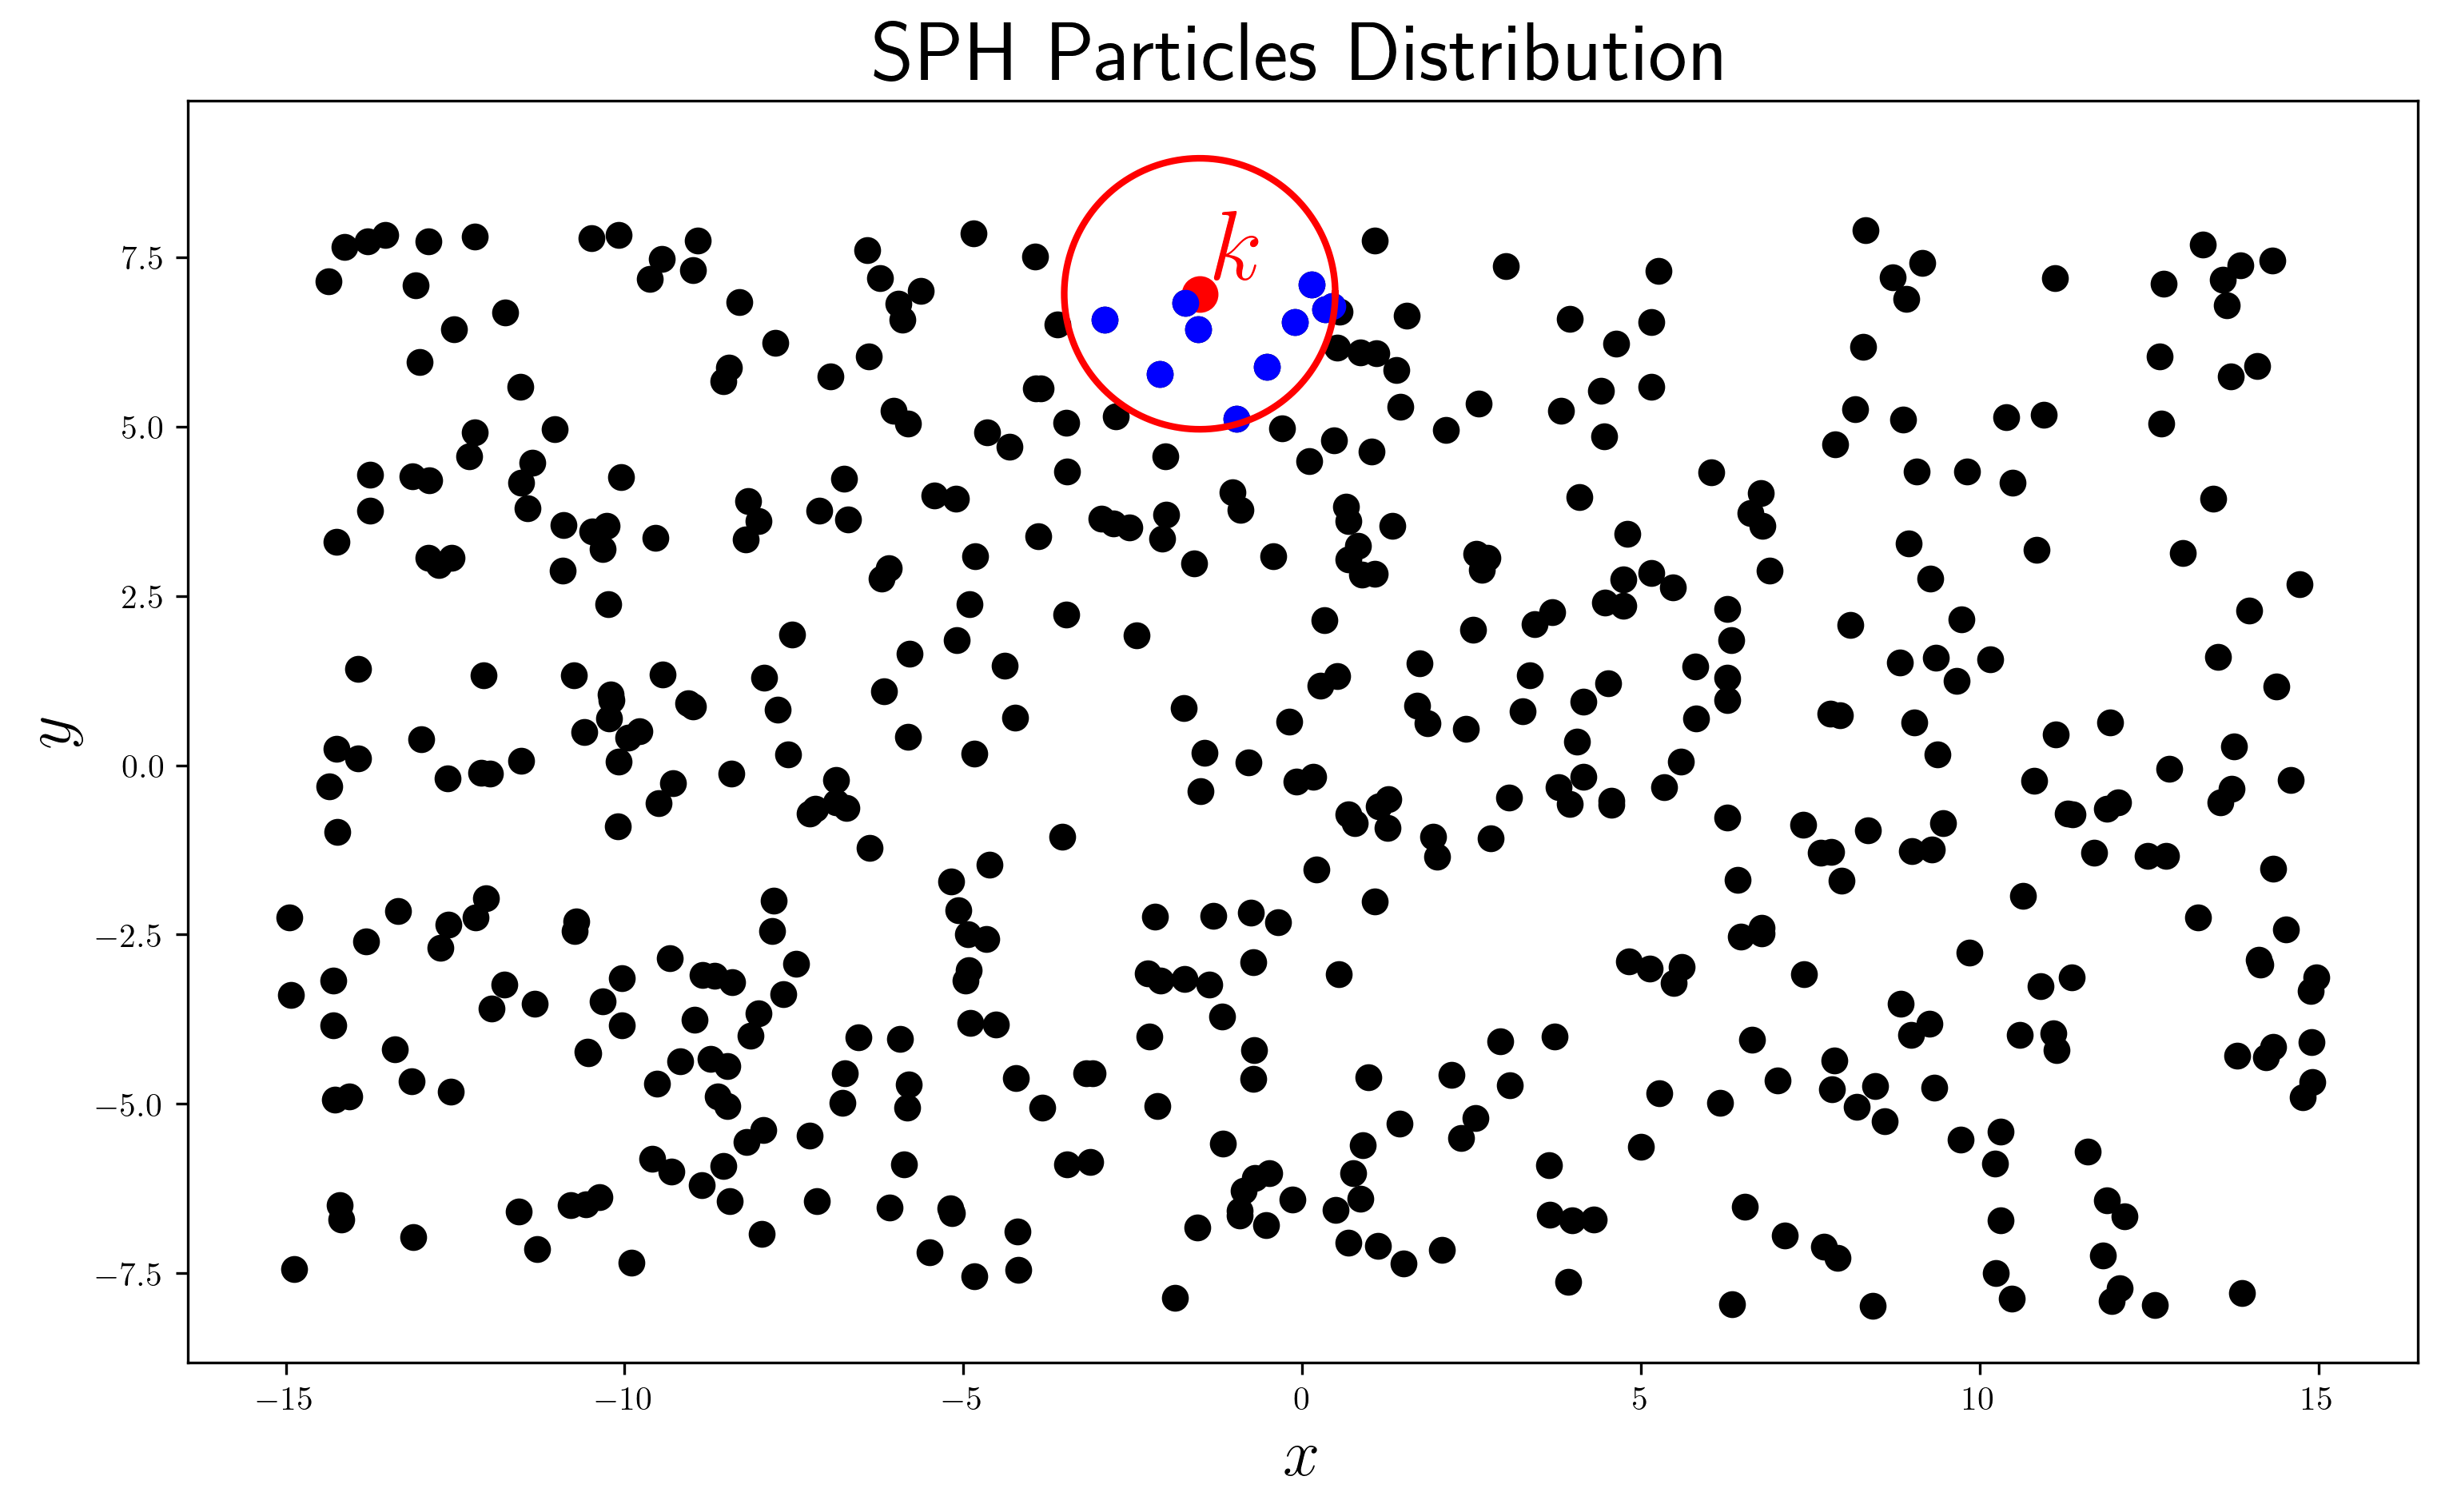
\includegraphics[width=0.7\textwidth]{images/sph_particles_distribution.png}
        \caption{物质点分布示意图}
        \label{fig:particles_distribution}
    \end{figure}
    而因为紧致性,事实上并不是所有的质点都会对质点 $k$ 处的值产生影响,
    仅在其核半径球内的质点才会对其产生影响,如图 \ref{fig:particles_distribution} 所示,
    编程中常用Hash表来存储这些质点,以加快计算速度。
    当然式 \ref{eq:scalar_field_approximation} 中的积分也有其他的格式,
    类似于传统FVM中的数值格式。
\end{frame}

\begin{frame}
    \begin{block}{各种格式的标量梯度的核函数插值}
        \begin{equation}
            \begin{aligned}
                \nabla u(\vec{r}_i) &= 
                    \sum_{j=1}^N
                    \frac{m_j}{\rho_j} u(\vec{r}_j)\frac{\vec{r}_i-\vec{r}_j}{r_{ij}}
                    \frac{\partial W_{ij}}{\partial r_{ij}}\\
                \nabla u(\vec{r}_i) &=
                    \frac{1}{\rho_i}\sum_{j=1}^N m_j [u(\vec{r}_j) - u(\vec{r}_i)]
                    \frac{\vec{r}_i-\vec{r}_j}{r_{ij}}\frac{\partial W_{ij}}{\partial r_{ij}}\\
                \nabla u(\vec{r}_i) &= \rho_i
                    \sum_{j=1}^N \frac{m_j}{\rho_j^2} 
                    \left[
                        \frac{u(\vec{r}_j)}{\rho_j^2} + \frac{u(\vec{r}_i)}{\rho_i^2}
                    \right]
                    \frac{\vec{r}_i-\vec{r}_j}{r_{ij}}\frac{\partial W_{ij}}{\partial r_{ij}}\\
            \end{aligned}
        \end{equation}
    \end{block}
\end{frame}

\subsection{控制方程和算法流程}

\begin{frame}
    在给出方程前首先需要注意的事情是SPH方法是基于拉格朗日描述的,
    对于不可压流体(一般用来求解不可压问题),
    Kochier与Bender \cite{koschier_smoothed_2020} 给出控制方程如下:
    \begin{equation}
        \begin{cases}
            &\nabla\cdot\vec{u} = 0\\
            &\rho \frac{\partial \vec{u}}{\partial t} = 
            -\nabla p + \mu \nabla^2 \vec{u} + \vec{f}
        \end{cases}
    \end{equation}
    他们给出了一套较为完整的算法流程,大致如下:
    \begin{itemize}
        \item 对所有粒子求解 $\frac{\partial \vec{u}}{\partial t}=\nu\nabla^2\vec{u}+\frac{1}{\rho}\vec{f}$ ;
        \item 根据不可压性质,求解 $\nabla p=\vec{0}$ ;
        \item 再次更新速度场 $\frac{\partial \vec{u}}{\partial t}=-\frac{1}{\rho}\nabla p$ ;
        \item 更新所有粒子位置 $\vec{x}_{\text{next}}=\vec{x}_{\text{curr}}+\vec{u}\Delta t$ 。
    \end{itemize}
\end{frame}

\begin{frame}
    \begin{figure}[H]
        \centering
        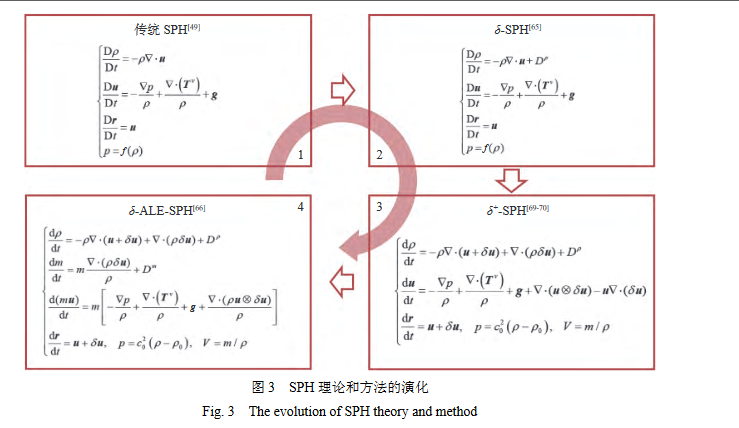
\includegraphics[width=0.8\textwidth]{images/sph离散方程.png}
        \caption{SPH方程离散形式的演化\cite{_sph_2022}}
    \end{figure}
    其中西工大黄晓婷\cite{_sph_2022-3}采用 $\delta^+$ SPH 方法求解翼型绕流问题。
    上述过程虽然看起来比较简单
    但实际在计算的过程中会涉及到很多问题,
    依目前查询文献结果来看,
    可能遇到的问题如下如质点质量分布的初始化\cite{tian_systematic_2017},
    自由表面捕捉问题\cite{_sph_2022-1},
    压力梯度精度不足导致的数值空腔\cite{_sph_2022-3}等。
\end{frame}

\subsection{边界条件的处理}

\begin{frame}
    SPH方法的边界条件处理是一个比较复杂的问题,
    一般来说,边界条件可以分为两类:自由边界和固壁边界。
    \begin{block}{自由边界}
        采用追踪法,即在计算过程中,
        将自由表面的粒子标记出来,然后在计算过程中,
        通过求解自由表面的法向加速度来更新自由表面的位置。
        这块在蒋肖蒙\cite{_sph_2022-1}的硕士毕业论文钟有描述,
        其构建了一套自由表面捕捉和重构的方法。
    \end{block}
    \begin{block}{固壁边界}
        一般镜像法,即在计算过程中,
        将固壁边界的粒子标记出来,然后在计算过程中,
        通过求解固壁边界的法向加速度来更新固壁边界的位置,
        但这种方法需要进行压力修正以避免粒子堆积。
        另外还有固定虚粒子法和改进固定虚粒子法,
        即用固定的假想粒子来代替固壁边界。
    \end{block}
\end{frame}

\begin{frame}
    \begin{figure}[H]
        \subfigure[自由表面捕捉与重构]{
            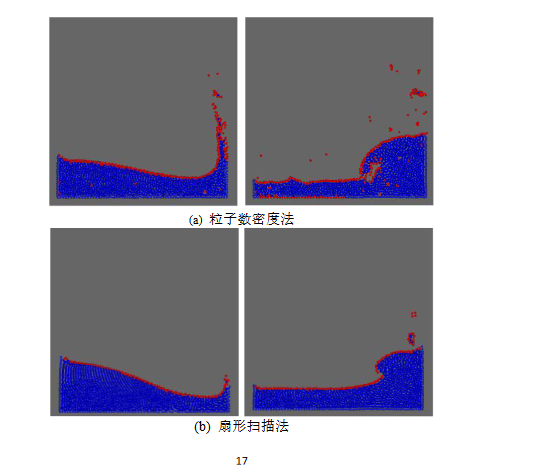
\includegraphics[width=0.42\textwidth]{images/surface_reconstruct.png}
        }
        \subfigure[固定边界虚粒子处理法]{
            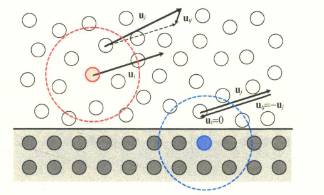
\includegraphics[width=0.52\textwidth]{images/fixed_bd.png}
        }
        \caption{两类常用边界处理方法}
    \end{figure}
\end{frame}